%
%	Documento de análisis (diagramas)
%

\documentclass[11pt, a4paper, twoside, titlepage]{article}
\usepackage[utf8x]{inputenc}
\usepackage[T1]{fontenc}
\usepackage[spanish, es-ucroman]{babel}
\usepackage{lmodern}
\usepackage{anysize}
\usepackage{fancyhdr}
\usepackage[none]{hyphenat}
\usepackage[colorlinks, linkcolor=red]{hyperref}
\usepackage{float}
\usepackage{lscape}
\usepackage{pdflscape}
\usepackage[doc=analisis]{isdiedral}

% Nombre del documento (para futuras referencias)
\newcommand*{\doctitle}{Diseño}
\newcommand*{\docversion}{1.0}


%%% Configuraciones %%%
\marginsize{2.5cm}{2cm}{2cm}{2cm}

% Usa como familia tipográfica por defecto "Sans"
\renewcommand{\familydefault}{\sfdefault}

% Establece la profundidad hasta la cual se numeran los elementos de sección
\setcounter{secnumdepth}{4}

% Establece la profundidad de niveles de sección que aparece en el TOC
\setcounter{tocdepth}{4}

% Configuración de los encabezados
\encabezadodiedral{\doctitle{} \docversion}
\pagestyle{fancy}

\renewcommand*{\thepage}{\sffamily \roman{page}}

\title{\doctitle\\\textsl{Airline Common Environment}}
\author{Grupo Diedral}

% Metadatos del pdf
\hypersetup{
pdfinfo={
	Author={Grupo Diedral},
	Title={\doctitle{} \docversion},
	Subject={Airline Common Environment},
	Keywords={diseño, UML, Airline Common Environment, Ingeniería del Software}
}
}

\begin{document}
	% Tabla de cambios
	\begin{tablacambios}
		1.0 & 28 de abril de 2013 & Todos & Versión inicial
	\end{tablacambios}

	% Cita inicial
	\fijacitainicial{Hay dos formas de elaborar un diseño software: una es hacerlo simple para que sea obvio que no hay deficiencias, la otra es hacerlo suficientemente complicado para que no haya deficiencias obvias. El primer método es mucho más difícil}{C.A.R. Hoare (1980)}

	% Portada
	\portadaace{\doctitle}{\docversion}

	\tableofcontents
	\newpage

	\iniciarnumeraciondiedral

	\begin{prologo}
		Este documento recoge la documentación generada durante la fase de diseño del proyecto.\\

		Esta información ha sido especificada por medio del \itshape{Lenguaje Unificado de Modelado} (UML).

	\paragraph*{Nota sobre herramientas empleadas:} para la elaboración de los diagramas se ha utilizado el\break programa {\normalfont BoUML} en su versión {\normalfont 4.23 patch 7 `ultimate'}.
	\end{prologo}

	\section{El paquete {\itshape Gestión Externa}}
		\subsection{Introducción}
			\parskip = .2cm
			La interfaz de gestión externa se ha implementado como una aplicación gráfica de escritorio utilizando la biblioteca gráfica {\itshape Swing} del lenguaje de programación {la \itshape Java}.

			Por un lado se encuentran las clases representantes de objetos del dominio (como \textit{Vuelo}, \textit{Billete}, \textit{Pasajero} \ldots) y otras clases artificiales que realizan funciones necesarias para la aplicación (siguiendo el criterio GRASP de la \textit{fabricación pura}), especialmente en lo concerniente al manejo y la persistencia de los datos.

			Otra parte de la aplicación la componen las clases relacionadas con la comunicación con el usuario por medio de la interfaz gráfica. El modelo consiste en una \textit{VentanaPrincipal} compuesta por varias clases auxiliares que contiene un marco intercambiable donde se muestran las diferentes pantallas correspondientes a los diferentes casos de uso. Al tratarse de la interfaz externa, la aplicación se ha diseñado con cierta apariencia de página web.

			Para la puesta en práctica del almacenamiento de los datos se ha utilizado la \textit{serialización} de Java con aquellos objetos que así lo requiren.
			

		\subsection{Diagrama de clases}

			\begin{figure}[H]\centering
				\vspace{2cm}
				\hspace{-2cm}
%				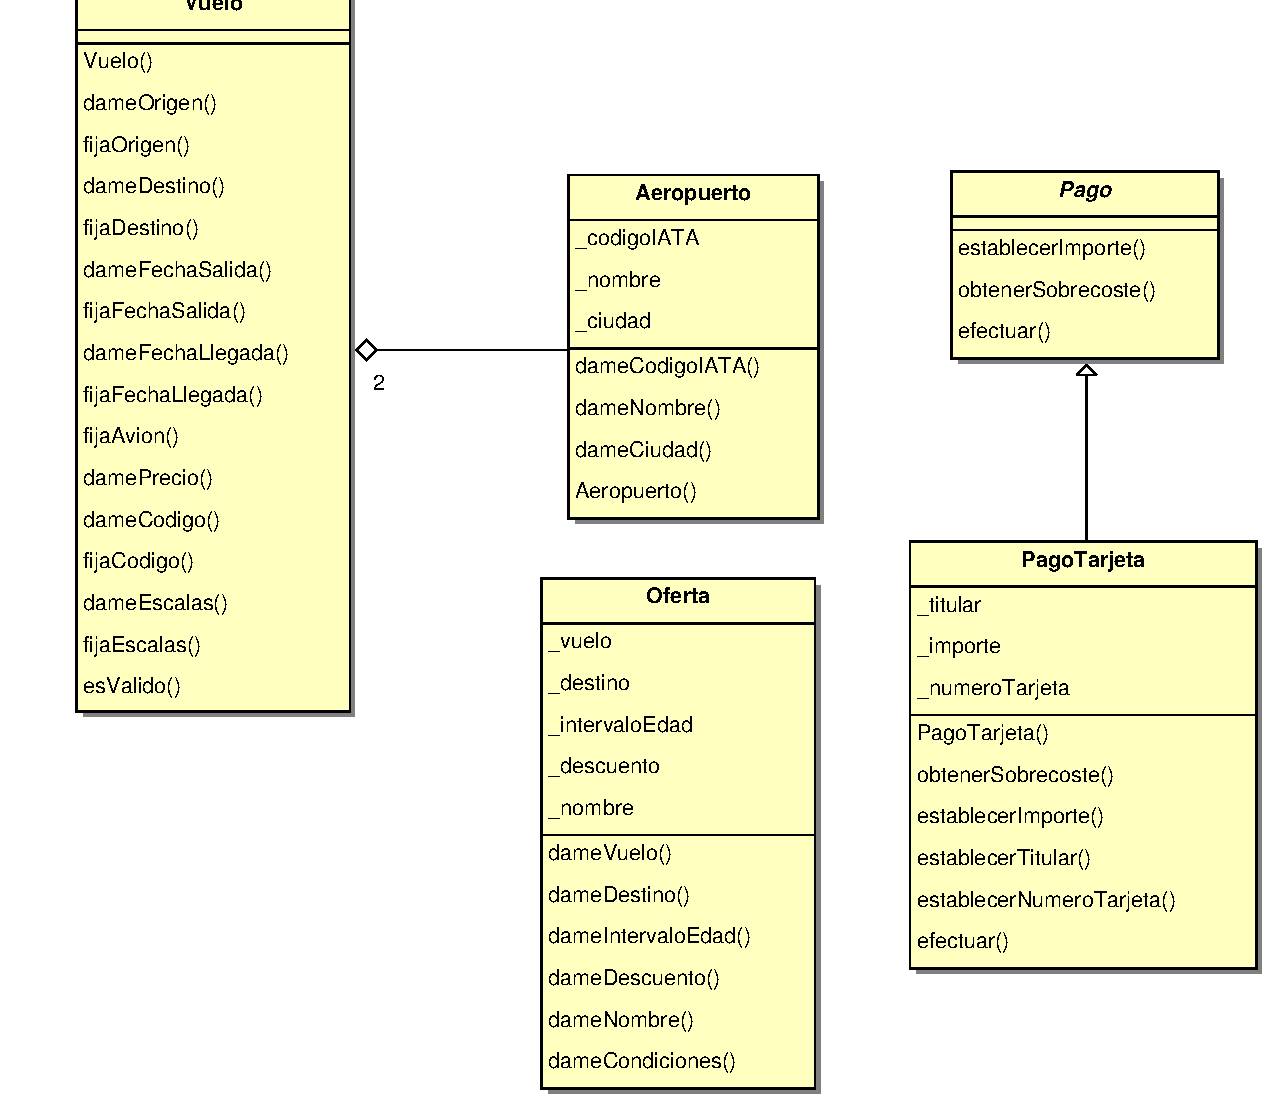
\includegraphics[scale=1]{diagramas/diagramaclases.pdf}
			\end{figure}

		\subsection{Diagramas de secuencia}

			\subsubsection{Acceder web}
				\begin{figure}[H]\centering
					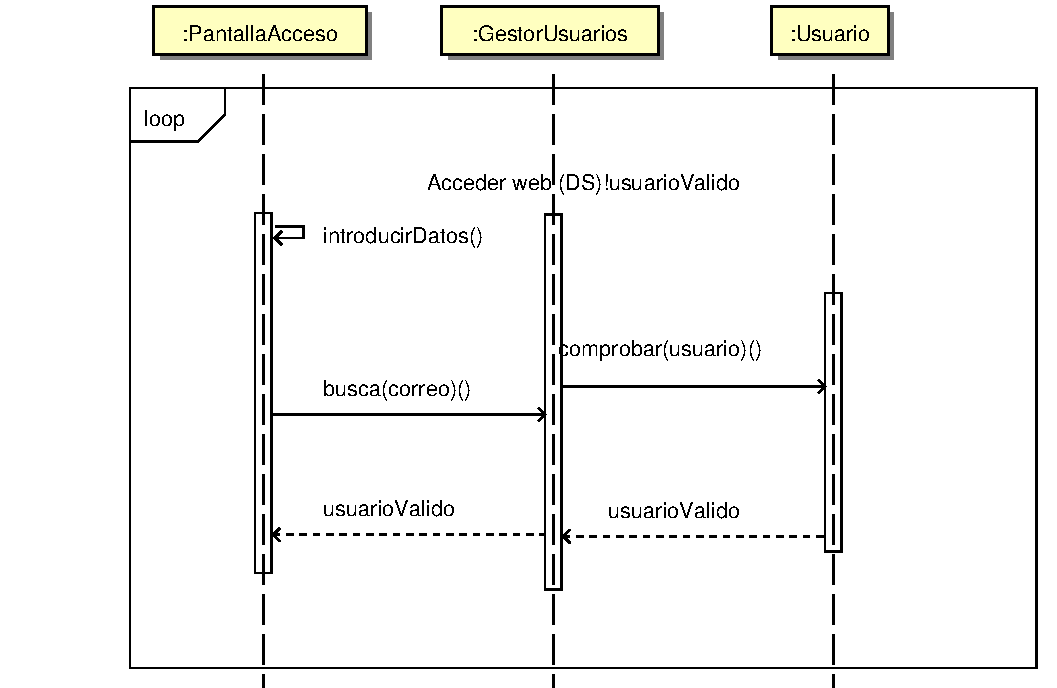
\includegraphics[scale=.7]{diagramas/accederweb.pdf}
				\end{figure}

			\subsubsection{Comprar billete}
				\begin{figure}[H]\centering
%					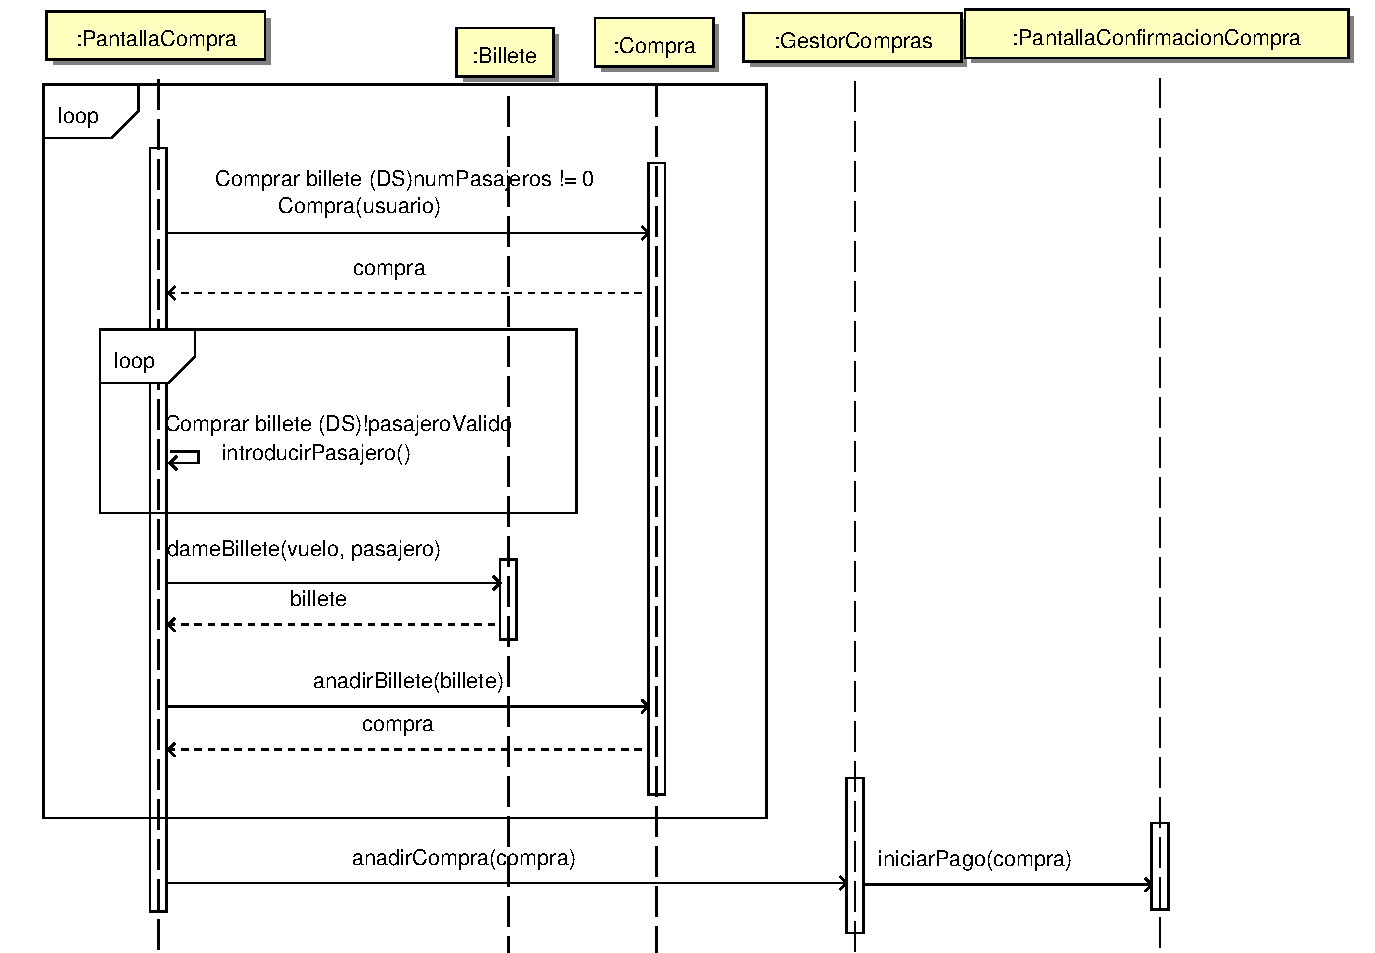
\includegraphics[scale=.7]{diagramas/comprarbillete.pdf}
				\end{figure}

			\subsubsection{Consultar oferta}
				\begin{figure}[H]\centering
%					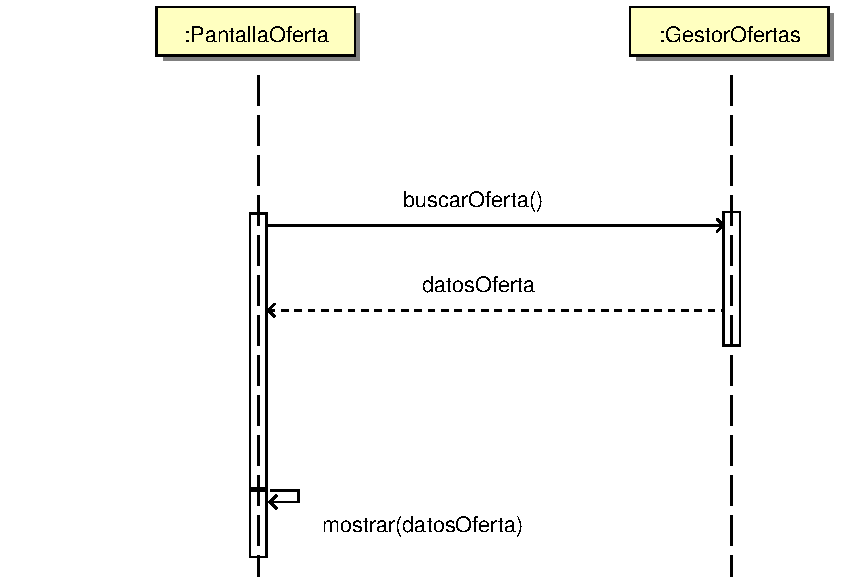
\includegraphics[scale=.7]{diagramas/consultaroferta.pdf}
				\end{figure}

			\subsubsection{Consultar vuelos}
				\begin{figure}[H]\centering
					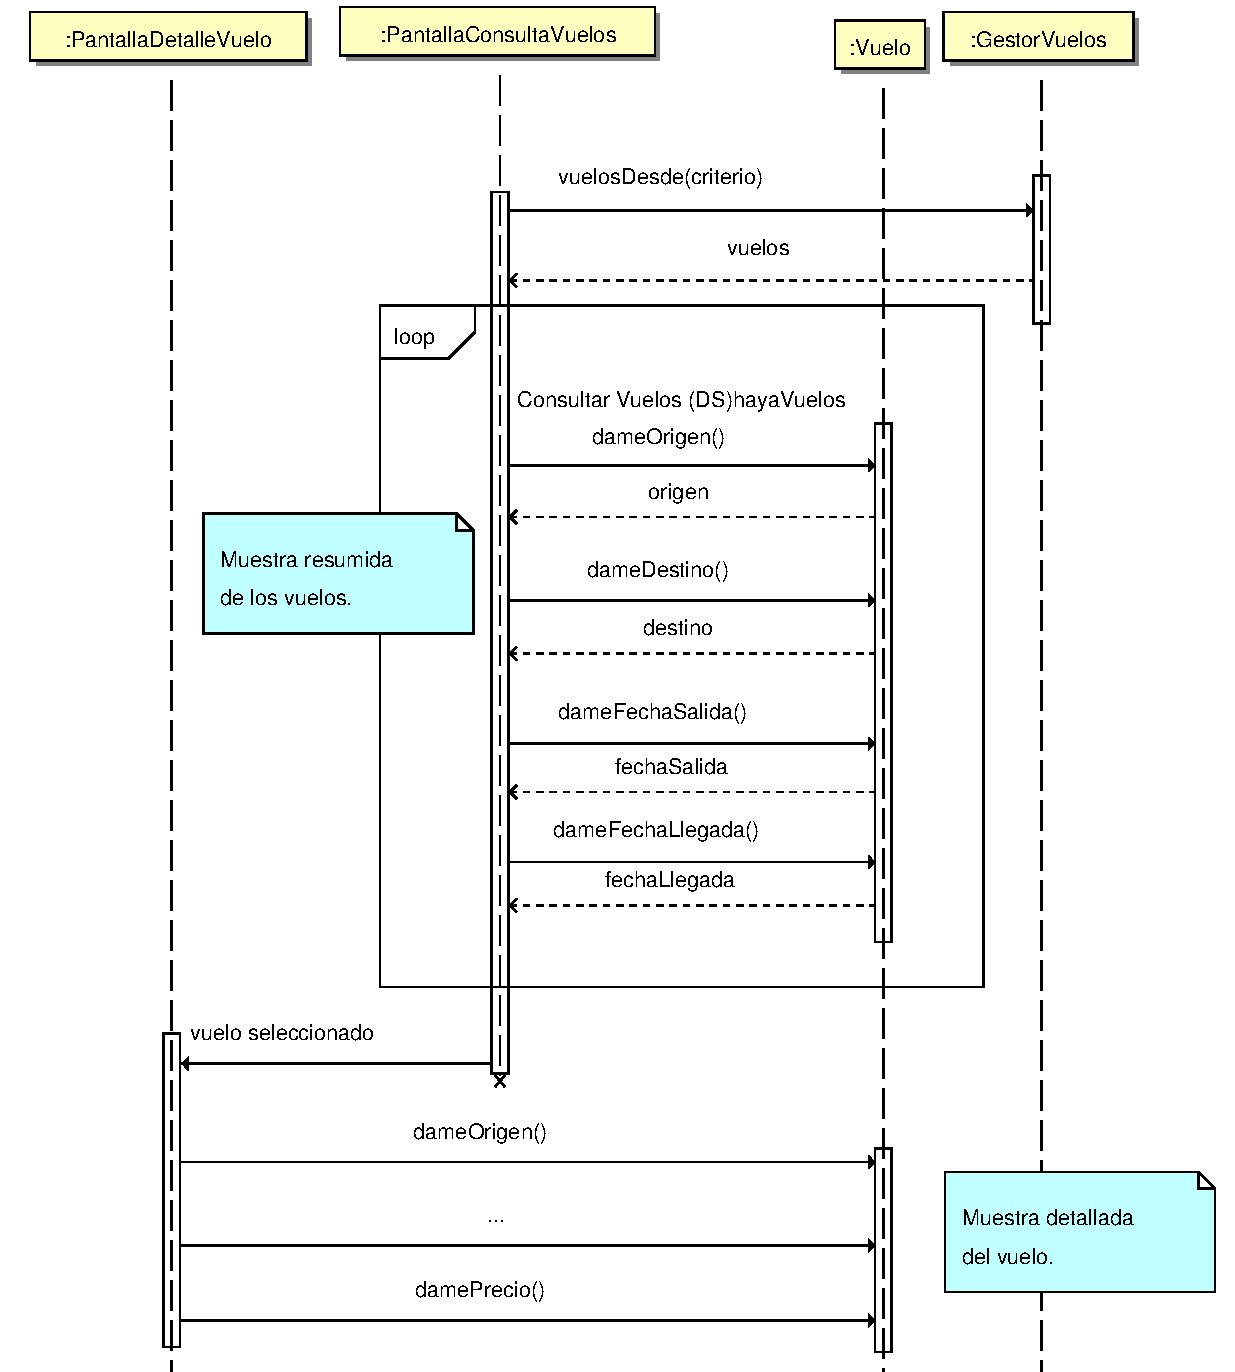
\includegraphics[scale=.7]{diagramas/consultarvuelos.pdf}
				\end{figure}

				La pantalla {\itshape PantallaConsultaVuelos} permite al usuario buscar vuelos por diferentes criterios (aeropuerto de salida, aeropuerto de llegada, fecha de salida, fecha de llegada, \ldots) y muestra los resultados de las búsquedas con la información básica que les corresponde. El usuario puede seleccionar una de las apariciones para ver una vista detallada del vuelo, con la información completa y poder desde allí acceder a la compra del billete.

				{\itshape GestorVuelos} representa un administrador de vuelos que permite obtener listas filtradas de entre los disponibles por medio de los criterios especificados.
			
			\subsubsection{Editar datos personales}
				\begin{figure}[H]\centering
					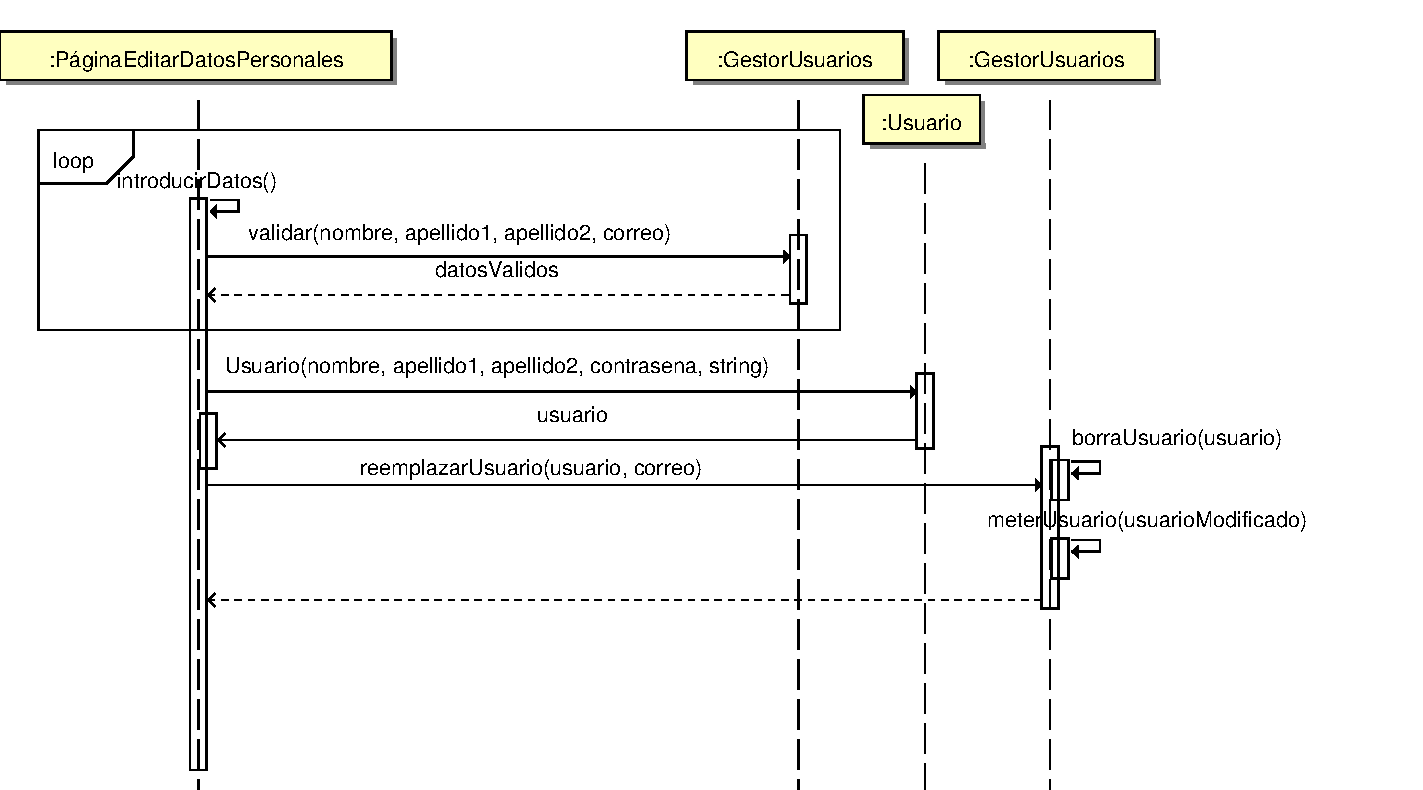
\includegraphics[scale=.7]{diagramas/editardatospersonales.pdf}
				\end{figure}


			\subsubsection{Iniciar pago billetes}
				\begin{figure}[H]\centering
					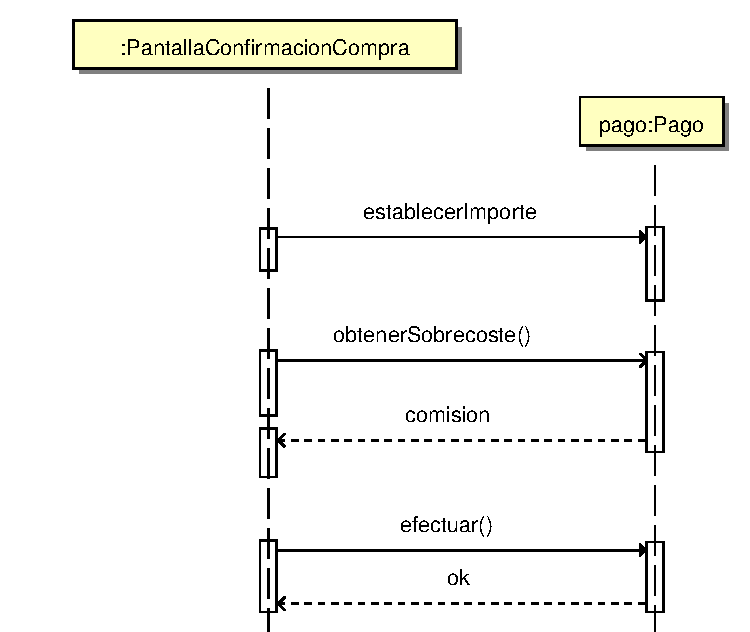
\includegraphics[scale=.7]{diagramas/iniciarpagobilletes.pdf}
				\end{figure}

			\subsubsection{Mostrar ofertas}
				\begin{figure}[H]\centering
					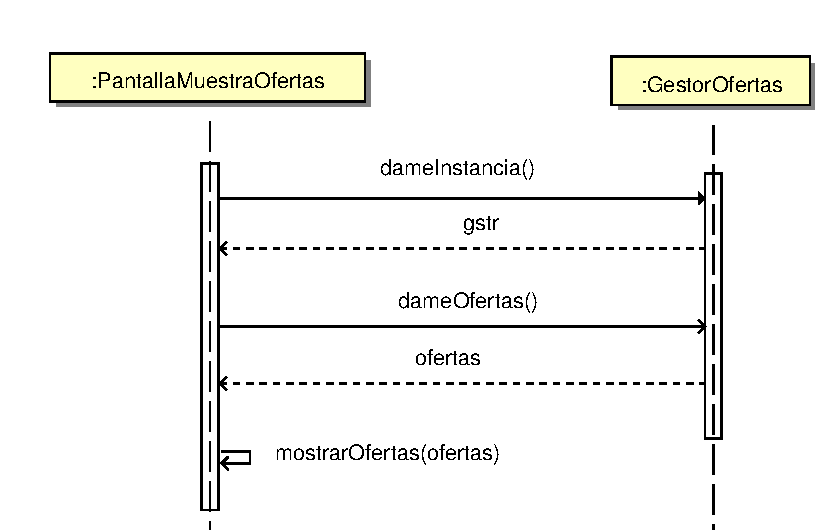
\includegraphics[scale=.7]{diagramas/mostrarofertas.pdf}
				\end{figure}

			\subsubsection{Realizar pago con tarjeta}
				\begin{figure}[H]\centering
					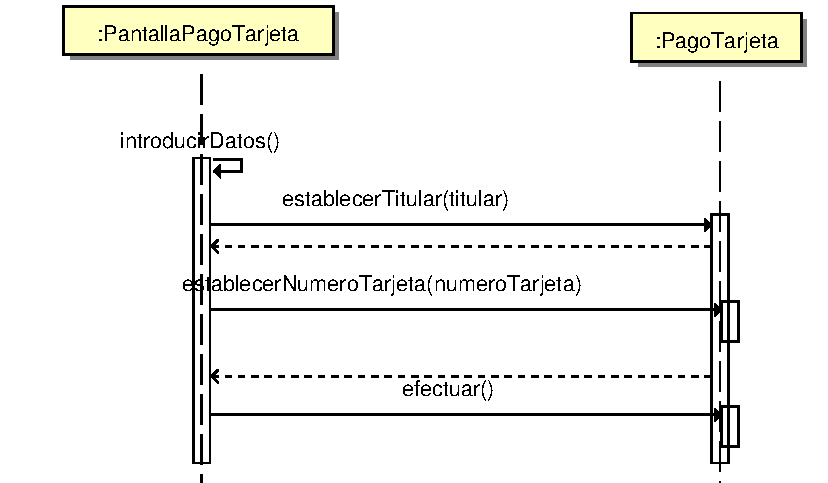
\includegraphics[scale=.7]{diagramas/pagotarjeta.pdf}
				\end{figure}

			\subsubsection{Presentar reclamación}
				\begin{figure}[H]\centering
					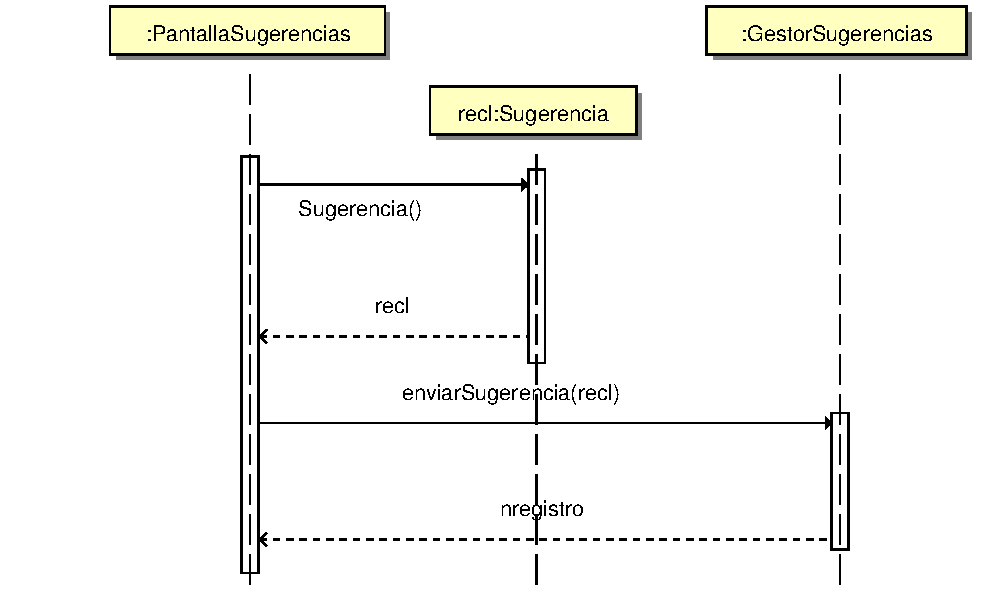
\includegraphics[scale=.7]{diagramas/presentarreclamacion.pdf}
				\end{figure}

				Por medio de la pantalla {\itshape PantallaSugerencias} el usuario expone su sugerencia, incluyendo con ella --de forma opcional-- su nombre y una dirección de contacto donde recibir respuesta. {\itshape PantallaSugerencias} construye una sugerencia ({\itshape recl}) con los datos aportados. La operación de construcción de {\itshape Sugerencia} puede dar lugar a errores si el mensaje de sugerencia es vacío o la dirección de correo electrónico de contacto no se ajusta al formato. Si no se producen esos hechos habrá construida una {\itshape Sugerencia} válida que será enviada a la compañía por medio de la clase {\itshape GestorSugerencias} que devolverá un número identificativo del registro que deberá ser mostrado al usuario para futuras alegaciones.

			\subsubsection{Registrarse}
				\begin{figure}[H]\centering
%					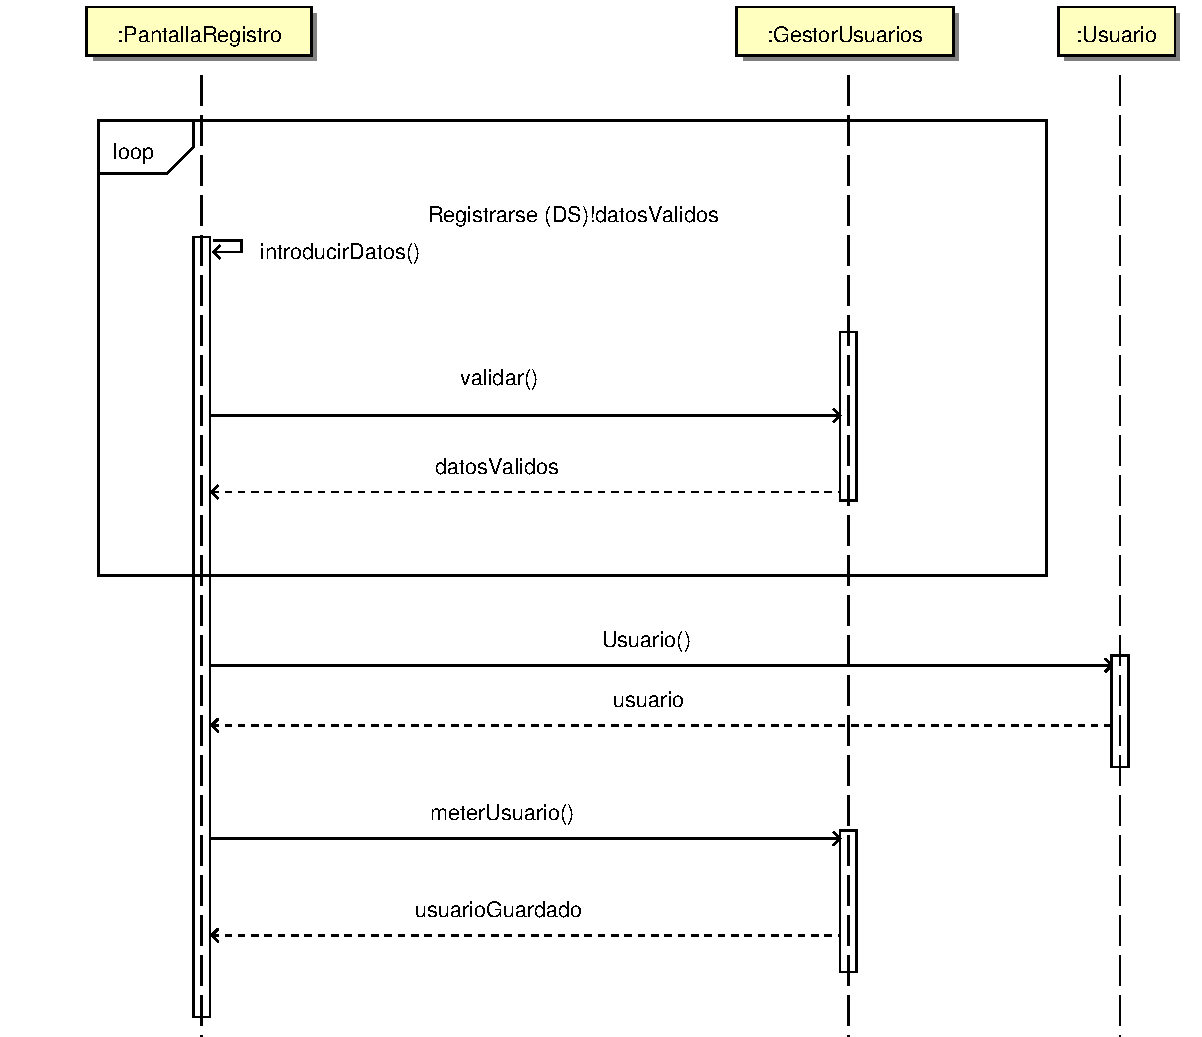
\includegraphics[scale=.7]{diagramas/registrarse.pdf}
				\end{figure}

			\subsubsection{Restablecer contraseña}
				\begin{figure}[H]\centering
%					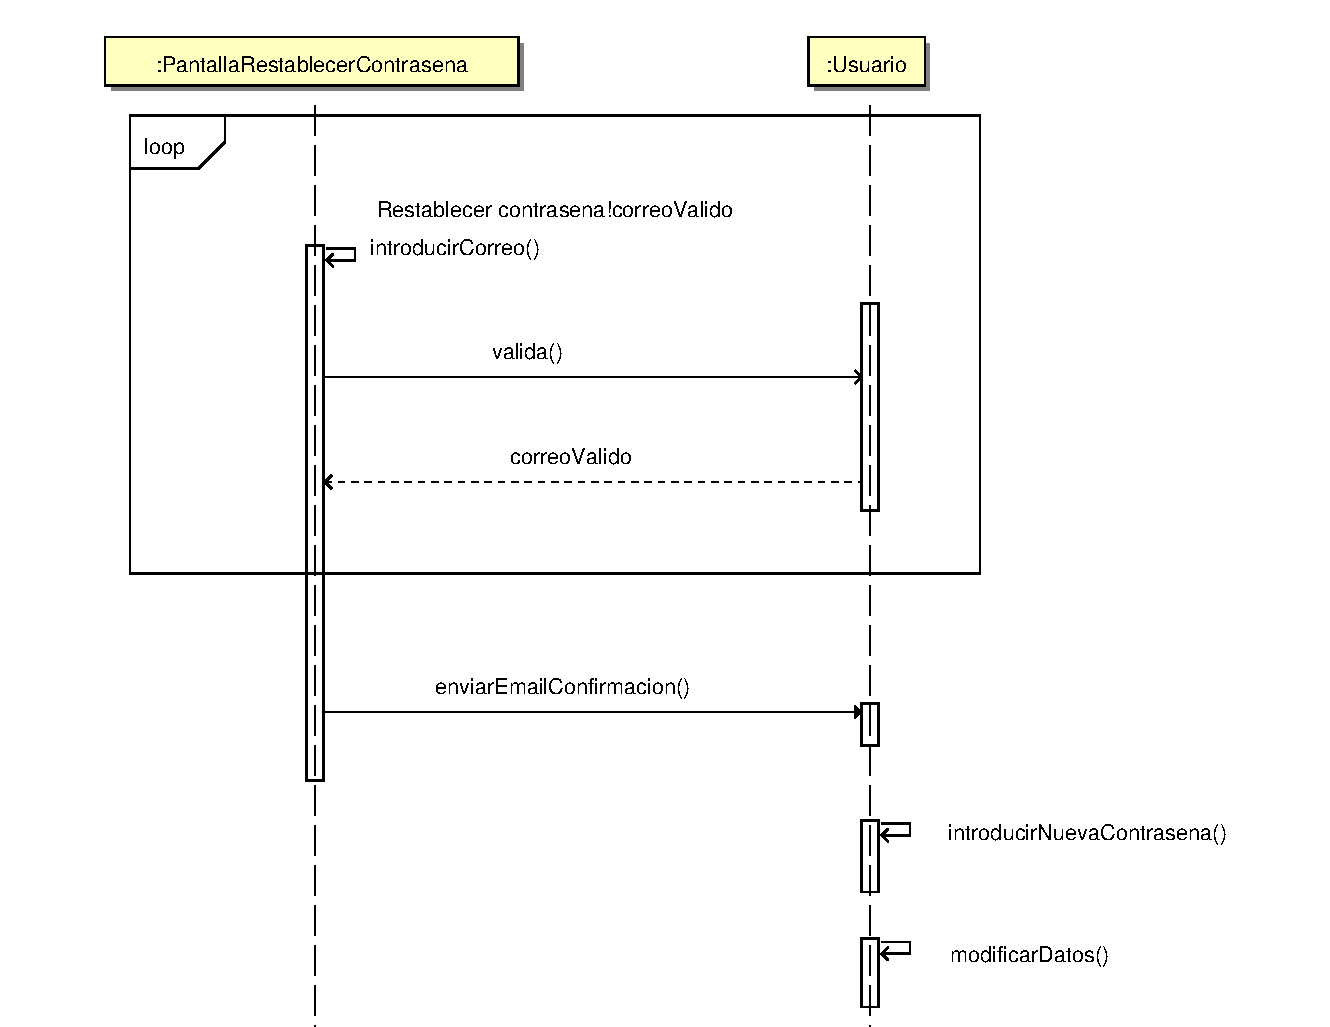
\includegraphics[scale=.7]{diagramas/restablecercontrasena.pdf}
				\end{figure}

			\subsubsection{Ver información de vuelo contratado}
				\begin{figure}[H]\centering
%					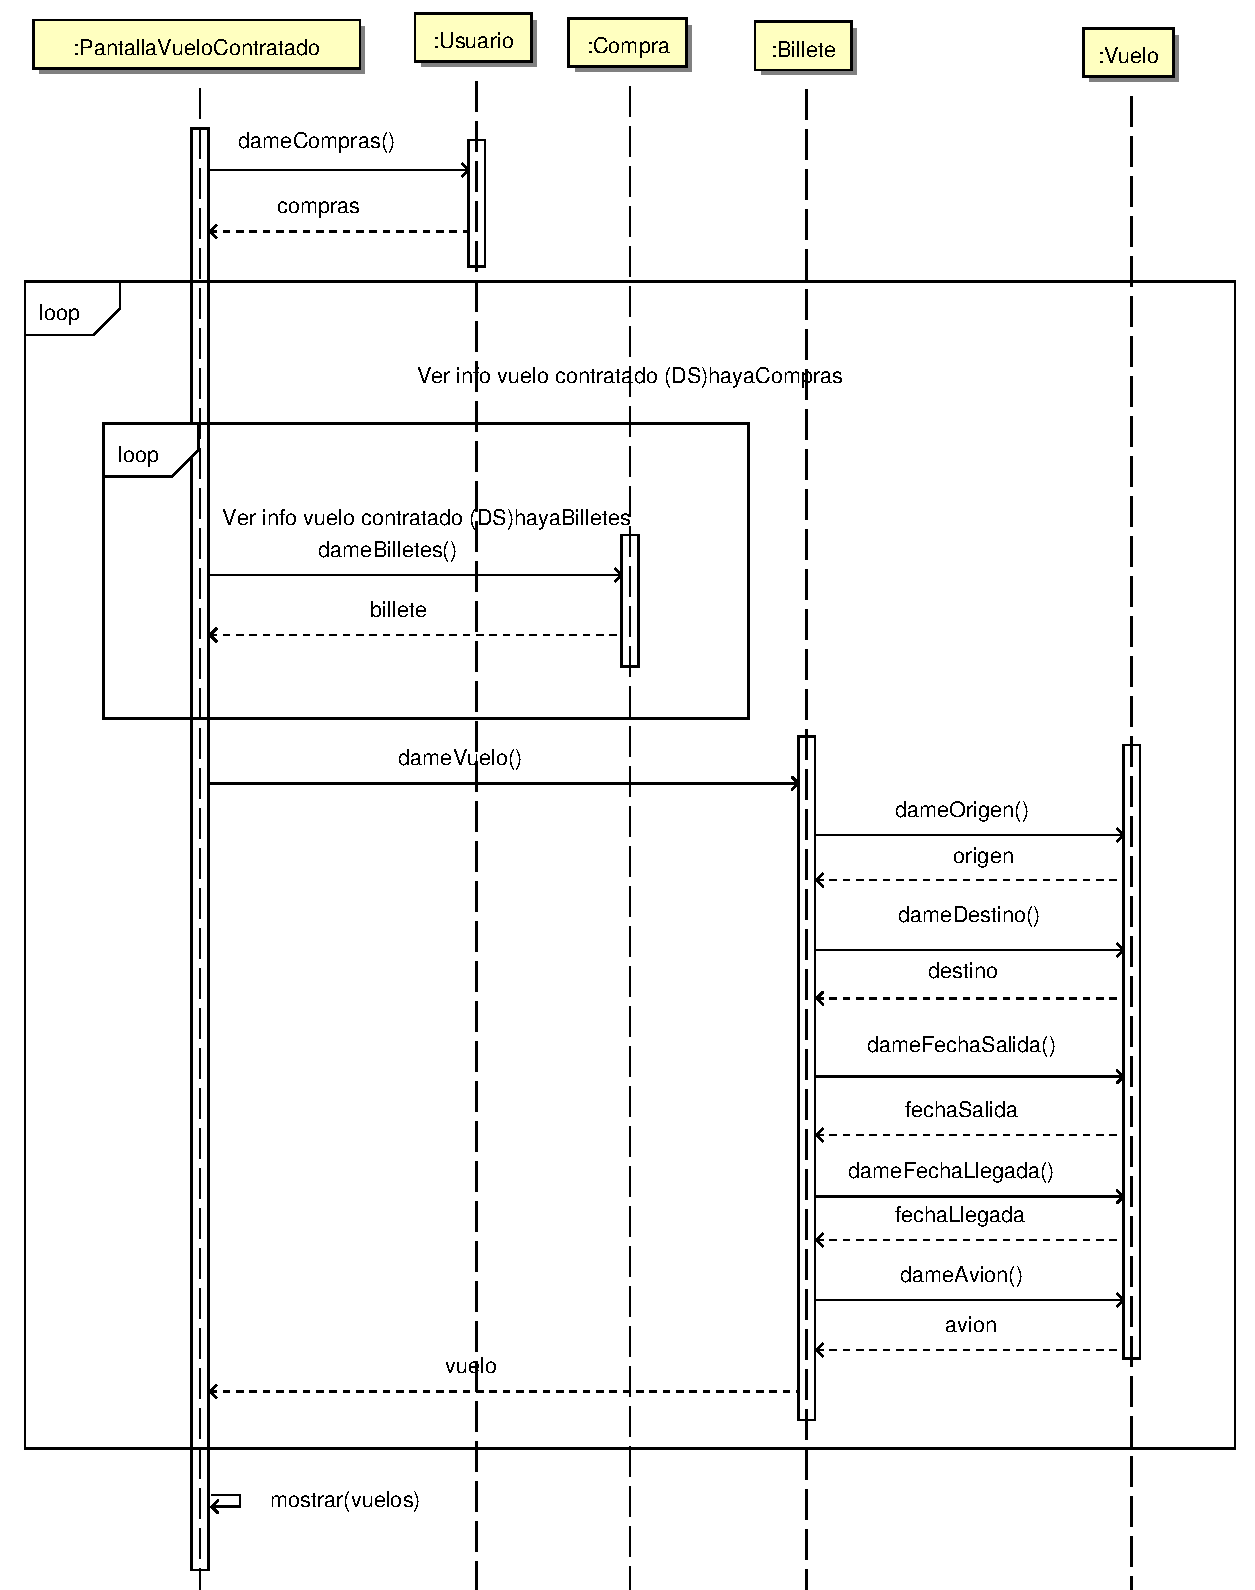
\includegraphics[scale=.7]{diagramas/verinfovuelocontratado.pdf}
				\end{figure}

	\subsection{Aplicación de patrones de diseño}
		\parskip = .2cm

		En el diseño de esta aplicación \software se han utilizado de forma intencionada o casual algunos patrones de diseño orientado a objetos que han sido explicados en clase.

		Para la asignación de responsabilidades y relaciones a las clases se ha intentado aplicar el patrón \textit{Experto}, reducir el acoplamiento y 	mantener una alta cohesión.

		A lo largo de toda la aplicación se puede observar el patrón GRASP denominado \textit{Polimorfismo}. Los ejemplos más notables son los métodos de pago (\textit{MetodoPago}) y las \textit{Pantalla}s asociadas a los casos de uso en la interfaz gráfica, casos que también son ejemplos del patrón \textit{Puente}.

		En la interfaz gráfica se recurre también al patrón \textit{Observer}, bien organizado por el propio \textit{Swing} (\textit{Java}), bien implementado para usos particulares.

		En las clases asociadas a la persistencia de los datos (en teoría, la comunicación con la base de datos; en la práctica, el control de archivos persistentes) se pone en práctica el modelo \textit{Solitario}, ya que es especialmente conveniente por la unicidad de la fuente de datos y la conveniencia de utilizar operaciones sobre instancias en lugar de métodos estáticos (por ejemplo la segunda posibilidad restringe las facilidades de serialización).

		Una interpretación del patrón \textit{Visitante} es utilizada en los criterios de búsqueda a los que se les hace recorrer una lista de candidatos, comprobando en cada uno de ellos si cumplen los criterios establecidos.

\end{document}
